This chapter introduces the Java programming language. It is primarily focused on description of its platforms and
specially on Java Standard Edition and its Application Programming Interface (API) which serves as the basis for Android
API described in Chapter~\ref{AndroidChapter}.

Section~\ref{JavaLangSection} presents the Java programming language, Java platforms are described in
Section~\ref{JavaPlatformsSection} and Section~\ref{JavaSESection} introduces Java Standard Edition and its main parts.

\section{Java language}\label{JavaLangSection}
Java~\cite{JavaBook, Java6Doc} is one of the most famous and most widely used computer programming languages in the
world. It is developed by Oracle Corporation and its application is widespread. Java is used for programming smart
cards, mobile and desktop applications, as well as large business and information systems. It is class based and object
oriented language which is managed by the Java Language Specification and together with the supporting runtime forms
programming environment.

The first public version of Java was released in 1996 and since this year, eight more versions was released. In 2010,
Java changed its owner from Sun Microsystems to Oracle Corporation. The latest version of Java (Java 8) was released in
2014.

\section{Java platforms}\label{JavaPlatformsSection}
Java is published in four platforms. Each platform provides tools for development and running programs written in Java
and consists of two main parts. The first part is Java Virtual Machine (JVM) which is connected to an~operating system
and thus Java programs can be executed. The second part is Java Application programming interface which provides many
public classes of standard Java libraries.

The following paragraphs briefly describe four platforms: Java Standard Edition (Java SE), Java Enterprise Edition
(Java EE), Java Micro Edition (Java ME) and Java Card.

\paragraph{Java Standard Edition}
Basic and the most famous platform which is designed for desktop and simple server application development. Currently,
the most recent version is Java SE 8.

\paragraph{Java Enterprise Edition}
Extension of Java SE that contains special libraries for developing and running enterprise software applications and
information systems. Java EE is based on Java SE 7 in the current version.

\paragraph{Java Micro Edition}
Subset of Java SE for application development for small devices such as microcontrollers, mobile phones, set-top boxes,
printers and other devices is called Java ME. Currently, the most recent version is Java ME 8.1.

\paragraph{Java Card}
This technology is designed for application development of smart cards or devices with limited memory and processing
capabilities. For example, it is used for SIM cards of mobile devices, plastic smart card for Automated teller machine
and similar devices. Last released version is Java Card 3.

\section{Java Standard Edition}\label{JavaSESection}
Java SE platform is distributed in two versions. The first version is Java Runtime Enviroment which is commonly used on
personal computers for running Java applications. The second version named Java Development Kit is used mostly for
application development. This platform has its own open-source implementation called OpenJDK~\cite{OpenJDK}.
Figure~\ref{JavaComponentsFigure} shows parts of Java SE Development Kit (JDK) distribution in comparison with Java SE
Runtime Environment (JRE) and in the following paragraphs, these components are briefly described.
\\
\begin{figure}[h!]
    \centering
    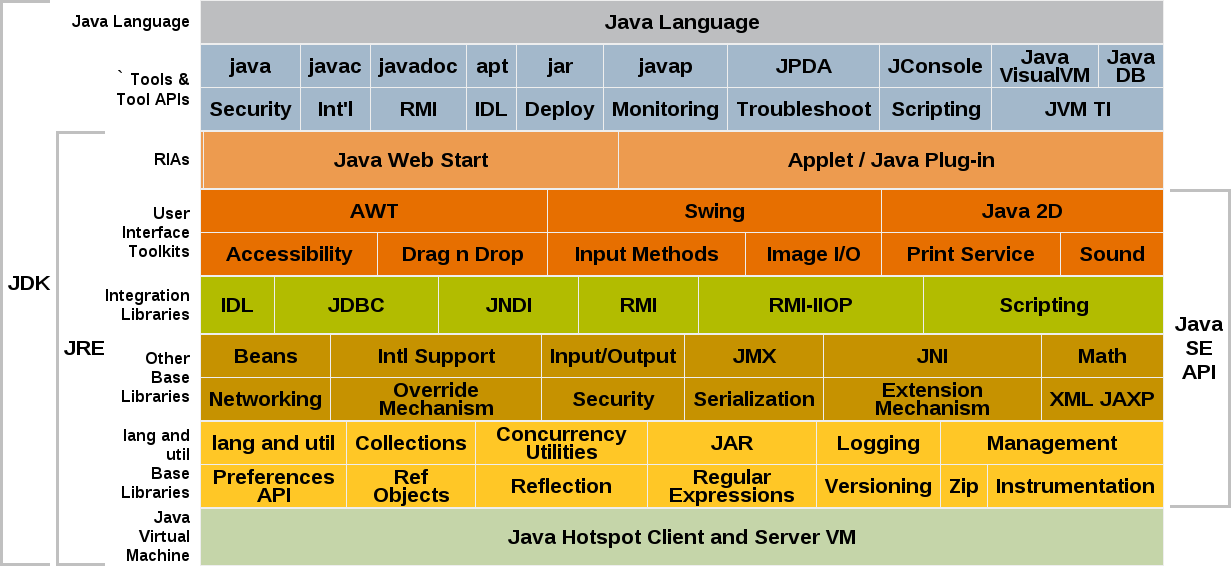
\includegraphics[scale=0.35]{fig/java_6_jdk.png}
    \caption{Components of the Java Standard Edition Development Kit 1.6~\cite{Java6Doc}.}
    \label{JavaComponentsFigure}
\end{figure}

\paragraph{Java SE Development Kit}
Java SE Development Kit is sometimes known as Software Development Kit (SDK). It is tool containing everything necessary
for developing Java application. The main part of JDK is JRE which is described below. Further, it contains the tools
to create and build applications (such as compiler, documentation generator, etc.), security, localization and other
tools. The last part of JDK is Java Language Specification which describes rules of this programming language.

\paragraph{Java SE Runtime Environment}
JRE is runtime environment for running Java applications. It consist from Java API, Java Virtual Machine and tools for
creating rich internet applications.

\paragraph{Java SE Application Programming Interface}
Java API is set of public classes of standard libraries. These libraries include packages for creating graphical user
interface, manipulation with databases, base language and utility libraries and many others.

\paragraph{Java Virtual Machine}
Java programs can not run without virtual machine. JVM is a~program that provides the runtime environment necessary for
executing of Java application. Figure~\ref{JavaLifecycleFigure} shows the lifecycle of Java program. It starts with
Java source code which is compiled to bytecode by \texttt{javac} compiler. Bytecode is an~instruction code and it is
stored in \texttt{.class} files. These files go through classloading mechanism to JVM and then are ready for execution
by the interpreter.
\\
\begin{figure}[h!]
    \centering
    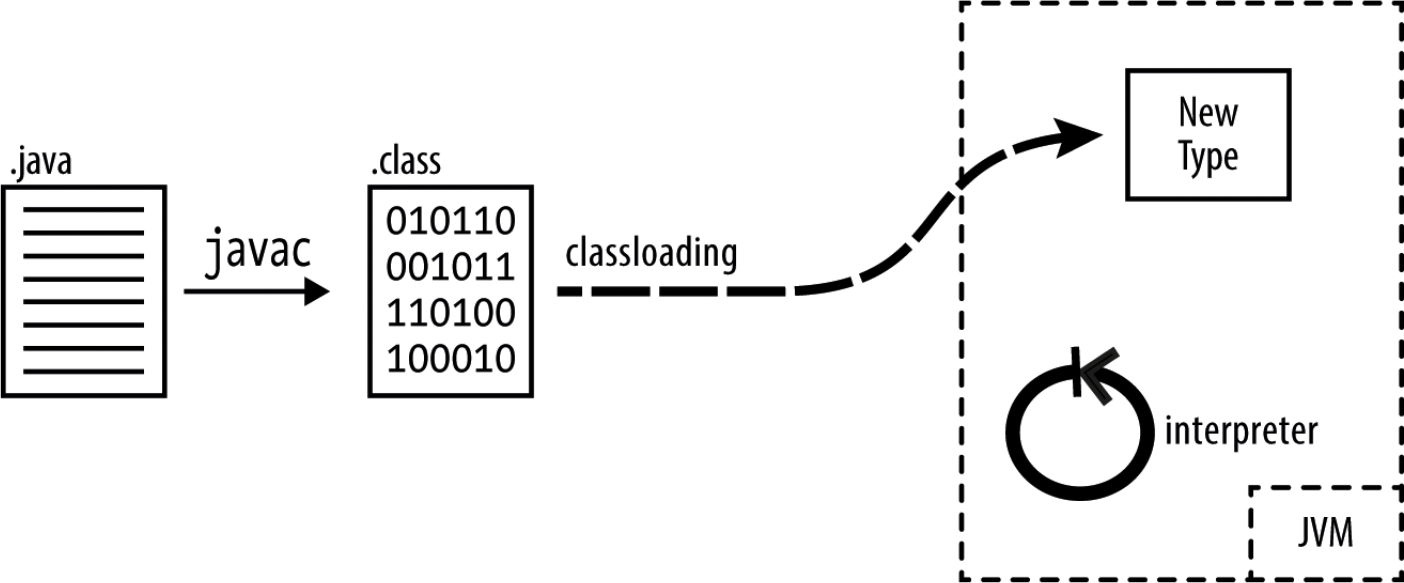
\includegraphics[scale=0.3]{fig/java_program_lifecycle.png}
    \caption{The lifecycle of a~Java program~\cite{JavaBook}.}
    \label{JavaLifecycleFigure}
\end{figure}
